\documentclass[10pt,a4paper]{article}

\usepackage[colorlinks=true,urlcolor=blue,linkcolor=blue]{hyperref}
\usepackage[utf8]{inputenc}
\usepackage[T1]{fontenc}
\usepackage[french]{babel}

\usepackage{pgf-umlsd}
\usepgflibrary{arrows}
\usepackage{fancyvrb}
\usepackage{tikz}

\usepackage{graphicx}
\usepackage{float}

\title{Cahier des besoins - Reversi}
\author{Guillaume CHUPIN, Benoit FAGET, Alexis PICHON, Julien PILLEUX}

\begin{document}
\maketitle
\newpage
\tableofcontents
\newpage

\section{Introduction}
\label{sec:intro}
Notre projet consiste en l'élaboration d'un joueur de Reversi complet, développé en suivant certaines règles, afin de pouvoir être confronté à d'autre implémentations au cours d'un tournoi prévu qui le confrontera au programme d'une seconde équipe de développement ayant reçu le même sujet.\\

Nous avions le choix entre le langage de programmation C et le C++, nous avons choisi d'utiliser le C++. Notre programme doit appliquer les algorithmes les plus fréquents pour un joueur de Reversi et doit utiliser au mieux les bitboards. Un bitboard est une structure de données qui est très efficace pour encoder un plateau de jeu tel que celui du Reversi. En effet, s'agissant d'un ensemble de bits, chaque bit peut correspondre à une case du plateau et indiquer la présence ou l'absence d'une pièce, ainsi on doit utiliser deux bitboards, un pour les pions blancs et un autre pour les pions noirs. L'interface utilisateur devant être purement en mode texte dans un bash, où les pions blanc seront représenté avec des \verb!O! et les pions noir avec des \verb!X!, on doit plutôt se concentrer sur le développement d'heuristiques propres au jeu. Le projet doit être essentiellement dirigé vers l'utilisation de techniques d'exploration d'arbre classiques telles que Minimax-$\alpha\beta$, Negamax, Negascout, MTD(f), Monte-Carlo Tree Search (MCTS), etc. Nous définirons lesquelles développer en premières ultérieurement.\\

Le jeu de Reversi est un jeu de stratégie au tour par tour opposant deux joueurs où tous les éléments sont connus et où le hasard n'a pas sa place. Chaque joueur possède des pions qu'il doit disposer sur le plateau, avec la possibilité de capturer les pions adverses, le but étant de terminer avec le plus grand nombre de pions. La partie commence avec le joueur noir et se termine lorsque plus aucun mouvement n'est possible pour chacun des deux joueurs. Le plateau de jeu est initialisé avec quatre pions, deux par joueur, posés au centre, comme le montre la Fig. \ref{fig:début_du_jeu}. Par défaut, la taille du plateau est de \verb!8x8!, mais il est possible de jouer avec un tableau de taille plus grande ou plus petite, tant que la largeur du plateau est égale a sa longueur.

\begin{figure}[H]    
\centering
\begin{BVerbatim}
  A B C D E F G H
1 _ _ _ _ _ _ _ _
2 _ _ _ _ _ _ _ _
3 _ _ _ _ _ _ _ _
4 _ _ _ O X _ _ _
5 _ _ _ X O _ _ _
6 _ _ _ _ _ _ _ _
7 _ _ _ _ _ _ _ _
8 _ _ _ _ _ _ _ _
\end{BVerbatim}
\caption {Initialisation du jeu avec un plateau de \texttt{8x8}.\label{fig:début_du_jeu}}
\end{figure}
\newpage
Un joueur peut placer un pion uniquement sur une case vide adjacente à un pion adverse, et si le pion ainsi posé permet la capture d'au moins un pion adverse. Pour capturer les pions adversaires, il faut que ceux-ci se retrouvent pris entre l'un de vos pions déjà présents et celui que vous vous apprêtez à poser sur le plateau. La capture de pions peut s'effectuer dans les huit directions à la fois (voir Fig. \ref{fig:aire_de_capture}).

\begin{figure}[H]    
\centering
\begin{tikzpicture}
\node (x) {X};
\node (r) at (0.8,0) {};
\node (ru) at (0.63,0.63) {};
\node (u) at (0,0.75) {};
\node (lu) at (-0.63,0.63) {};
\node (l) at (-0.8,0) {};
\node (ld) at (-0.63,-0.63) {};
\node (d) at (0,-0.75) {};
\node (rd) at (0.63,-0.63) {};

\draw[->] (x) -- (r);
\draw[->] (x) -- (ru);
\draw[->] (x) -- (u);
\draw[->] (x) -- (lu);
\draw[->] (x) -- (rd);
\draw[->] (x) -- (d);
\draw[->] (x) -- (ld);
\draw[->] (x) -- (l);
\end{tikzpicture}
\caption {Aire de capture d'un pion.\label{fig:aire_de_capture}}
\end{figure}
\tikzstyle{block}=[rectangle, draw, text width=6em, text centered, rounded corners, minimum height=4em]

Depuis, qu'un programme a battu le champion du monde d'Othello à 6-0, en 1997\cite{CK06}, on considère que les programmes sont meilleures que les humains pour le jeu d'Othello.

\section{Description et analyse de l'existant}

\subsection{Programmes}
\label{sec:programmes}
Pour qu'un programme puisse décider d'un coup à jouer, il lui faut calculer quelles peuvent être les réponses de son adversaire et ainsi se projeter quelques coups dans l'avenir. On stocke ces informations dans un arbre où les noeuds correspondent à un état du jeu et les arcs à des coups joués (voir Fig. \ref{fig:exemple_arbre}).\\

\begin{figure}[H]    
\centering
\begin{tikzpicture}
\node[block, label=left:{Tour noir}] (a) at (3,5) {\begin{BVerbatim}
  A B C D 
1 _ _ _ _ 
2 _ O X _ 
3 _ X O _
4 _ _ _ _

\end{BVerbatim}
};

\node[block, label=left:{Tour blanc}] (b) at (-1,0) {\begin{BVerbatim}
  A B C D 
1 _ _ _ _ 
2 X X X _ 
3 _ X O _
4 _ _ _ _

\end{BVerbatim}
};

\node[block] (c) at (2,0) {\begin{BVerbatim}
  A B C D 
1 _ X _ _ 
2 _ X X _ 
3 _ X O _
4 _ _ _ _

\end{BVerbatim}
};

\node[block] (d) at (5,0) {\begin{BVerbatim}
  A B C D 
1 _ _ _ _ 
2 _ O X _ 
3 _ X X X
4 _ _ _ _

\end{BVerbatim}
};

\node[block] (e) at (8,0) {\begin{BVerbatim}
  A B C D 
1 _ _ _ _ 
2 _ O X _ 
3 _ X X _
4 _ _ X _

\end{BVerbatim}
};

\node[block, label=left:{Tour noir}] (f) at (2,-4) {\begin{BVerbatim}
  A B C D 
1 _ _ _ _ 
2 _ O X _ 
3 _ O X X
4 _ O _ _

\end{BVerbatim}
};

\node[block] (g) at (5,-4) {\begin{BVerbatim}
  A B C D 
1 _ _ _ _ 
2 _ O X _ 
3 _ X O X
4 _ _ _ O

\end{BVerbatim}
};

\node[block] (h) at (8,-4) {\begin{BVerbatim}
  A B C D 
1 _ _ _ _ 
2 _ O O O 
3 _ X X X
4 _ _ _ _

\end{BVerbatim}
};

\draw[->] (a) -- node [text width=2em,midway,above] {A2} (b);
\draw[->] (a) -- node [text width=2em,midway,above] {B1} (c);
\draw[->] (a) -- node [text width=3em,midway,above] {D3} (d);
\draw[->] (a) -- node [text width=4em,midway,above] {C4}(e);
\draw[->] (d) -- node [text width=2em,midway,above] {B4} (f);
\draw[->] (d) -- node [text width=3em,midway,above] {D4} (g);
\draw[->] (d) -- node [text width=4em,midway,above] {D2}(h);
\end{tikzpicture}
\caption {Exemple d'arbre partiel d'état de jeu de profondeur deux.\label{fig:exemple_arbre} }
\end{figure}

Un programme qui pourrait ainsi prévoir tous les coups possibles pourrait facilement savoir quels coups jouer pour s'assurer la victoire, mais de part le nombre grandissant de coups possibles, il n'est pas envisageable de le faire dans un temps restreint. En effet, la complexité d'une telle recherche devient exponentielle et est de l'ordre de \begin{math}10^h\end{math}\cite{And07}, où h est la profondeur de l'arbre. Un plateau plus grand implique aussi plus de possibilités avec une partie plus longue. Il faut donc trouver un moyen d'obtenir de bons résultats sans explorer entièrement l'arbre de recherche des coups possibles.\\

La grande majorité des algorithmes utilise la méthode Minimax, ou une de ses variantes, pour trouver le meilleur coup à jouer dans l'arbre de jeu. Minimax est une technique qui part du principe que l'adversaire joue également de manière optimale, ainsi dans l'exploration on va essayer de maximiser nos bons coups tout en minimisant les bons coups adverses. Afin de déterminer les chances de gagner pour le joueur avec un certain coup, Minimax utilise une fonction d'évaluation, qui attribue à un état de jeu une note représentant a quel point l'état du jeu est intéressant.\\

Cette fonction d'évaluation se base principalement sur deux principes du jeu :\\

\begin{itemize}
\item \textbf{Stabilité des pions}: Un pion est stable si l'adversaire ne peut pas le reprendre pour le restant de la partie. Par exemple dans la Fig. \ref{fig:bord_stable}, tous les pions du plateau sont stables.\\

\begin{itemize}
\item \textbf{Bord stable}: Les quatre coins du plateau de jeu sont des positions stables et une fois une de ces positions prise. Le programme essaye d'obtenir un bord entièrement composé de pions stables lui appartenant. Dans la Fig. \ref{fig:bord_stable}, on peut voir un bord stable sur la gauche de la grille.

\begin{figure}[H]    
\centering
\begin{BVerbatim}
  A B C D E F
1 X _ _ _ _ X
2 X _ _ _ _ _
3 X _ _ _ _ _
4 X _ _ _ _ X
5 X _ _ _ X X
6 X _ _ X X X
\end{BVerbatim}
\caption{Exemple de bord stable.\label{fig:bord_stable}}
\end{figure}

\item \textbf{Stabilité interne}: Un pion se retrouvant entre des pions adverses est stable. Par exemple, dans la Fig. \ref{fig:stabilité_interne}, on peut voir que le joueur noir représenté par un 'X' peut effectuer une insertion en jouant en 'C1', le joueur blanc représenté par un 'O' ne pourra pas reprendre ce pion. Au tour suivant, quelque soit le coup du joueur blanc, le joueur noir pourra jouer en 'A1' et ainsi obtenir un des coins si désirés.

\begin{figure}[H]    
\centering
\begin{BVerbatim}
  A B C D E F
1 _ O _ O O _
2 _ _ O O O _
3 _ _ X _ _ _
4 _ _ _ _ _ _
5 _ _ _ _ _ _
6 _ _ _ _ _ _
\end{BVerbatim}
\caption{Exemple de stabilité interne.\label{fig:stabilité_interne}}
\end{figure}
\end{itemize}

\item \textbf{Mobilité}: Avoir un grand choix de coups est assez important étant donné que cela augmente les chances d'avoir de bons coups, tandis qu'avoir un faible nombre de coups entraînera inéluctablement vers de mauvaises décisions, voir pire vers aucune décision possible et dans ce cas la défaite est quasiment assurée. L'idéal est donc d'avoir un grand choix de coups, tout en réduisant le nombre de coups de l'adversaire (et ainsi réduire ses chances de victoire).\\

De plus, faire le dernier coup est assez avantageux puisque cela permet de prendre des pions qui ne seront jamais repris de part la fin de la partie, ainsi il peut être intéressant, si le coup final n'est pas notre, d'essayer de l'obtenir. Comme le joueur noir commence et qu'il y a un nombre pair de cases, c'est donc au joueur blanc que revient ce dernier coup, ainsi le joueur noir souhaitant obtenir ce dernier coup devra donc faire passer un tour au joueur blanc.\\

Mais cette notion de dernier coup existe aussi avant la fin de la partie. En effet, vers la fin de la partie, sur le plateau, il apparaît différentes zones où cette technique de dernier pourra également être utilisée. Par exemple, dans la Fig. \ref{fig:mobilité}, le joueur noir a la possibilité d'obtenir un dernier coup local en 'E6', alors que s'il décide de jouer en 'A2', il laisserait la possibilité au joueur blanc de faire un dernier coup local en 'A1'.
\begin{figure}[H]    
\centering
\begin{BVerbatim}
  A B C D E F
1 _ O O O _ _
2 _ X O X _ O
3 O X O X O O
4 O X X X X O
5 X X X O O O
6 O O O O _ O
\end{BVerbatim}
\caption {Exemple du principe de mobilité. C'est au joueur noir de jouer\label{fig:mobilité}}
\end{figure}
\end{itemize}

\subsubsection {Iago}

Dans les années 1980, un programme nommé Iago\cite{Ros81} est développé. Ce dernier optimise la recherche du prochain coup en limitant la recherche à un certain nombre de coups dans le futur, nombre déterminé par le temps alloué pour ledit coup. Il utilise également la technique d'exploration d'arbre Minimax-$\alpha\beta$. Minimax-$\alpha\beta$ est une amélioration de Minimax permettant de réduire le nombre de noeuds. En effet, certains sous-arbres dont l'on peut déjà savoir qu'il ne nous mènerons pas vers un meilleurs résultat que les sous-arbres déjà explorés ne seront pas considérés. Ainsi l'ordre dans lequel les branches sont évaluées devient important, Iago organise donc ses noeuds dans l'ordre croissant pour chaque recherche.\\

La fonction d'évaluation dont hérite Iago a été faite "à la main". En effet, ils ont testé plusieurs variations, basées sur les principes vus précédemment, en les faisant s'affronter les unes contre les autres et ont gardé la meilleure.

\subsubsection{Bill}
%% TODO: Voir si on garde cette section.
Peu après la création de Iago, le programme Bill\cite{LM86} est lui aussi développé, ce dernier arrive à vaincre Iago à chaque fois. Il est assez similaire à Iago, mais borne la valeur de retour de Minimax, ce qui permet d'exclure plus de branches, mais le risque reste que si la borne a été mal choisie la recherche retourne une valeur incorrect. Pour parer à cela, il suffit de regarder si la valeur retournée correspond à une des bornes, ainsi on sait si le résultat se situe en dehors de ces bornes.\\

Il utilise également une table de hashage pour stocker les meilleurs coups obtenus et profite du temps que son adversaire met à jouer pour la mettre à jour (alors que Iago se contentait d'attendre le coup de l'adversaire).

\subsubsection{Logistello}

Dans les années 1990, un programme nommé Logistello\cite{Bur95a} est développé. Ce dernier utilise également la technique d'exploration d'arbre Minimax-$\alpha\beta$. Ce qui fait sa particularité sont ses extensions et l'amélioration de sa fonction d'évaluation.\\

Une extension nommée ProbCut\cite{Bur95b} vient s'intégrer au programme Logistello et le rend bien plus performant. En comparaison d'un humain se servant de son expérience pour exclure certaines possibilités peu ou pas pertinentes, l'algorithme Minimax-$\alpha\beta$ cherche dans presque l'intégralité de l'arbre de jeu. L'extension ProbCut permet d'exclure des sous-arbres probablement pas très pertinents de la recherche en profondeur à une certaine hauteur dans l'arbre de jeu, le temps ainsi sauvé est utilisé pour rechercher plus profondément dans les sous-arbres restants.\\

Une amélioration de cette extension nommée Multi-ProbCut\cite{Bur97a} permettant l'exclusion d'encore plus de sous-arbres rend le programme encore plus performant. Cette amélioration utilise l'algorithme Negamax qui est une variante de Minimax pouvant être plus rapide, l'utilisation de NegaScout peut être une autre amélioration.\\

En 1997, après amélioration de sa fonction d'évaluation, le programme Logistello a joué une série de parties l'opposant à Takeshi Murakami, un champion du monde d'Othello, qui s'est terminée par une victoire écrasante de 6 parties à 0 pour Logistello. Le champion du monde explique que malgré une dernière partie parfaite de sa part, le programme a su sortir des coups juste inimaginables pour un être humain. Un récit de cette incroyable rencontre a été rédigé par Michael Buro, le développeur de Logistello, en personne\cite{Bur97b}.


\newpage
\section{Besoins fonctionnels}
\label{sec:besoins_fonctionnels}

\subsection{Grille de jeu}
\label{board}

Les cases en abscisses doivent être numérotées à l'aide de lettres, les cases en ordonnées à l'aide de chiffres. La grille par défaut doit être de dimensions \verb!8x8!. Les cases vides de la grille doivent être représentées à l'aide du caractère '\_', le joueur blanc doit être représenté par un 'O' et le joueur noir par un 'X'. Les cases où le joueur courant peut effectuer son prochain coup peuvent être représentées par '*'. Ce plateau de jeu doit être implémenté à l'aide de deux bitboards, comme expliqué précédemment (voir Fig. \ref{fig:exemple_board}).

\begin{figure}[H]    
\centering
\begin{BVerbatim}
  A B C D E F
1 _ _ _ _ _ _
2 _ _ * _ _ _
3 _ * O X _ _
4 _ _ X O * _
5 _ _ _ * _ _
6 _ _ _ _ _ _  
\end{BVerbatim}
\caption{Exemple d'affichage.\label{fig:exemple_board}}
\end{figure}

\subsection{Informations supplémentaires}
Par défaut, le programme lance le jeu en mode utilisateur contre utilisateur.\\
Si l'entrée de l'utilisateur est invalide, alors on affiche un message d'erreur et on propose une nouvelle saisie.\\
Si les options et/ou paramètres passés au programme ne sont pas valides, alors on affiche un message d'erreur et on propose d'essayer l'option d'aide.\\
Si le fichier de sauvegarde passé en paramètre n'existe pas ou n'est pas au bon format, alors on affiche un message d'erreur et on quitte le programme.

\subsection {Déroulement d'une partie}
\label{sec:déroulement_partie}

% Diagrammes de séquences
\begin{figure}[H]
\centering
\begin{sequencediagram}
% Instances
\newthread[blue]{user}{User} %[couleur]{nom 'variable'}{nom affichage}
\newthread[green]{game}{Reversi} %[distance]
\tikzstyle{inststyle}+=[bottom color=white, top color=white, rounded corners=3mm]
\newinst[4]{board}{Board} 

% Instanciation Plateau
\begin{messcall}{user}{./reversi}{game} %{source}{affichage}{destination}
\begin{call}{game}{create\_board()}{board}{update\_display()} %{source}{affichage}{destination}{retour}
\end{call}
\end{messcall}
\begin{sdblock}{Run loop}{The main loop}
  % Le joueur joue un coup
    \mess{user}{Play move}{game} % L'utilisateur choisi une case
    \begin{call}{game}{play\_move()}{board}{update\_display()} % Le jeu passe la chaîne correspondante au plateau
      \begin{call}{board}{check\_if\_valid()}{board}{valid} % Le plateau vérifie la validité du mouvement
      \end{call}
    \end{call}

% La machine joue à son tour
  \begin{call}{game}{ia\_play\_move()}{board}{update\_display()} % Normalement pas besoin de vérifier (si on code ça bien)
  \end{call}

% Le joueur décide de quitter
  \mess{user}{Enter 'q'}{game}
  \mess{game}{Ask save}{user}
  \mess{user}{Enter 'y'}{game}
  \begin{call}{game}{save\_game()}{board}{}
  \end{call}
\end{sdblock}
\end{sequencediagram}
\caption{Diagramme séquentiel de déroulement d'une partie.\label{fig:diagramme_partie}}
\end{figure}

\subsection{Liste des fonctionnalités}
\label{sec:fonctionnalités}

La fonction \verb!check_is_valid_()! va vérifier si l'entrée de l'utilisateur correspond à un coup légal, c'est à dire un coup dans les bornes du plateau, et conformes aux règles du \verb!Reversi! (Voir section \ref{sec:intro}). Si le joueur choisi un coup illégal, le programme demande alors à l'utilisateur de re-saisir un coup.\\
% Début nouvelle partie post TD1
\begin{itemize}
\item Le programme se présente sous la forme d'une exécutable pouvant se lancer via un bash par la ligne de commande \verb!./reversi!. Cette ligne de commande peut s'accompagner d'options modifiant le comportement du programme, que nous détaillerons dans la suite de cette liste.
\item L'entrée de l'utilisateur est insensible à la casse.
\item Lorsque le jeu est lancé, l'affichage du plateau est accompagné des règles du jeu ainsi qu'une explication rapide des commandes dont l'utilisateur dispose pour sélectionner un mouvement.
\item Le programme questionne l'utilisateur sur le choix de son prochain mouvement. L'entrée de l'utilisateur est alors une chaîne de caractères commençant par un numéro représentant l'ordonnée de la case et se terminant par une lettre correspondant à l'abscisse de cette même case. Dans l'exemple de la figure \ref{fig:exemple_board}, la chaîne de caractères \verb!2C! correspond à un coup légal.
\item Lorsque l'utilisateur entre une coordonnée étant hors du plateau, étant déjà occupée par un pion, ou n'étant pas un coup possible selon les règles du \verb!Reversi!, le programme signal alors que l'entrée est erronée, puis re-demmande à l'utilisateur de choisir un mouvement. Le cas où l'utilisateur rentre des données totalement non conformes à ces règles est aussi prit en compte.
\item Le programme peut être quitté à tout moment lorsque l'utilisateur saisi la lettre\verb!'q'! à la place de coordonnées valides.
\item Si l'utilisateur le souhaite, le programme peut sauvegarder l'état de la partie actuelle dans un fichier \verb!ASCII!. La sauvegarde présente sur sa première ligne le caractère correspondant au prochain joueur qui devait jouer au moment ou la partie est interrompue. Les lignes en dessous présentent alors l'état de la partie avec le positionnement des pions des deux joueurs (voir fig. \ref{fig:exemple_save}).
\item Un fichier de sauvegarde conformes au règles citées ci-dessus peut être utilisé pour charger une partie plutôt que d'en commencer une nouvelle, lors du lancement du programme.  Lancer le programme avec un fichier de sauvegarde valide passé en paramètre permet de charger une partie correspondant à la sauvegarde décrite par le fichier.
\begin{figure}[H]    
\centering
\begin{BVerbatim}
X
_ _ _ _ _ _
_ _ _ _ _ _
_ _ O X _ _
_ _ X O _ _
_ _ _ _ _ _
_ _ _ _ _ _ 
\end{BVerbatim}
\caption {Exemple de fichier de sauvegarde.\label{fig:exemple_save}}
\end{figure}

\item Le programme contient un mode compétition. Au lancement, l'option \verb!-c! ou \verb!--contest! suivit d'un fichier de sauvegarde. Le coup suivant calculé pour l'état de jeu passé en paramètre est affiché.
\item La taille du plateau de jeu doit être modifiable. Au lancement, l'option \verb!-s! ou \verb!--size!, suivit d'une valeur entre 1 et 5, fait varier la taille du plateau de 2 à 10 cases (voir Fig. \ref{fig:exemple_taille}). Par défaut, la grille affichée sera de dimensions
\verb!8x8!.

\begin{figure}[H]    
\centering
\begin{BVerbatim}
  A B C D
1 _ _ _ _
2 _ _ _ _
3 _ _ _ _
4 _ _ _ _    
\end{BVerbatim}
\caption {Exemple de grille générée avec l'option \textsc{-s 2}.\label{fig:exemple_taille}}
\end{figure}

\item Lors du lancement du programme il est possible de décider du rôle que va jouer l'intelligence artificielle grâce aux options suivantes.
\begin{description}
\item [-w, --white] Pour indiquer que l'IA jouera les pions blancs.
\item [-b, --black] Pour indiquer que l'IA jouera les pions noirs.
\item [-a, --all] Pour indiquer que l'IA jouera les deux camps.
\end{description}
\item L'utilisateur peut décider de jouer une partie contre un autre joueur lorsqu'il ne précise pas de rôle pour l'intelligence artificielle. Lorsqu'il décide de faire ainsi, chaque joueur décident, à leur tour, de leur mouvement en précisant les coordonnées voulues.
\item Le programme dispose alors de plusieurs intelligences artificielles différentes, ce qui permet de les faires jouer entre elle afin de déterminer la quelle d'entre elles est la plus performante. 
\item La version du programme est affichable avec l'option de lancement \verb!-V! ou \verb!--version!. 
\item Le mode verbeux est activable au lancement du programme avec l'option \verb!-v! ou \verb!--verbose!.
\item Une aide est disponible pour l'utilisateur grâce à l'option \verb!-h! ou \verb!--help!, elle liste l'ensemble des options du programme ainsi que leur description.
\item Le programme dispose d'une structure d'arbre de coups possibles tel que décrit par la figure \ref{fig:exemple_arbre}. Cette structure permettant de choisir le coup optimal en se basant sur une prédiction des coups futurs. L'intelligence parcours cet arbre pour extraire la configuration du jeu optimale.
\item L'intelligence artificielle dispose d'une fonction d'évaluation telle que décrite dans la section \ref{sec:programmes}. Cette fonction est capable de détecter la stabilité d'une case (voir sous-section \ref{sec:programmes}). Elle est aussi en mesure de détecter la mobilité associée à une case (voir sous-section \ref{sec:programmes}).
\end{itemize}
% Fin nouvelle partie post TD1.

%%%%%%%%%% Partie avant le TD1 %%%%%%%%%%
% \textbf{Lancer une nouvelle partie de Reversi entre deux utilisateurs :}\\
% \begin{itemize}
% \item Lancer le programme sans option dans une console de type bash ;
% \item Afficher un message de bienvenue et des explications sur le déroulement de la partie (voir \ref{board}) ;\\
% \item Initialiser la grille de jeu avec ses dimensions par défaut (voir \ref{board}) ;
% \item Déterminer les mouvements possibles pour le joueur en cours ;
% \item Mettre à jour la grille de jeu avec les mouvements possibles ;
% \item Afficher la grille de jeu ;\\
% \item (*) Proposer à l'utilisateur de saisir son mouvement ou de quitter la partie (voir \ref{board}) ;
% \item Vérifier que la saisie est valide, retourner à l'étape précédente si ce n'est pas le cas ;\\
% \end{itemize}
% Si l'utilisateur décide d'un mouvement à réaliser :
% \begin{itemize}
% \item Vérifier que le mouvement est valide, retourner à l'étape précédente si ce n'est pas le cas ;
% \item Mettre à jour la grille de jeu avec le mouvement fraîchement réalisé ;
% \item Terminer le tour et changer de joueur ;
% \item Déterminer les mouvements possibles pour le joueur en cours;
% \item Mettre à jour la grille de jeu avec les mouvements possibles ;
% \item Afficher la grille de jeu ;
% \item Si la partie se termine, afficher le vainqueur et quitter le programme.
% Sinon, retourner à l'étape (*) ;\\
% \end{itemize}
% Si l'utilisateur décide de quitter la partie :
% \begin{itemize}
% \item Proposer à l'utilisateur de sauvegarder l'état de la partie en cours avant de quitter (voir \ref{save}) ;
% \item Vérifier que la saisie est valide, retourner à l'étape précédente si ce n'est pas le cas ;
% \item Si souhaité, sauvegarder l'état de la partie en cours dans un fichier (voir \ref{save}) ;
% \item Quitter le programme ;
% \end{itemize}
% \newpage

% \textbf{Lancer une nouvelle partie de Reversi entre l'utilisateur et l'ordinateur :}\\
% \begin{itemize}
% \item Lancer le programme avec l'option -b ou -w dans une console de type bash (voir \ref{options}) ;
% \item Afficher un message de bienvenue et des explications sur le déroulement de la partie (voir \ref{board}) ;\\
% \item Initialiser la grille de jeu avec ses dimensions par défaut (voir \ref{board}) ;
% \item Déterminer les mouvements possibles pour le joueur en cours ;
% \item Mettre à jour la grille de jeu avec les mouvements possibles ;
% \item Afficher la grille de jeu ;\\
% \end{itemize}
% (*) Si c'est au tour de l'utilisateur :
% \begin{itemize}
% \item Proposer à l'utilisateur de saisir son mouvement ou de quitter la partie (voir \ref{board}) ;
% \item Vérifier que la saisie est valide, retourner à l'étape précédente si ce n'est pas le cas ;
% \end{itemize}
% Si l'utilisateur décide d'un mouvement à réaliser :
% \begin{itemize}
% \item Vérifier que le mouvement est valide, retourner à l'étape précédente si ce n'est pas le cas ;
% \item Mettre à jour la grille de jeu avec le mouvement fraîchement réalisé ;
% \item Terminer le tour et changer de joueur ;
% \item Déterminer les mouvements possibles pour le joueur en cours ;
% \item Mettre à jour la grille de jeu avec les mouvements possibles ;
% \item Afficher la grille de jeu ;
% \item Si la partie se termine, afficher le vainqueur et quitter le programme.
% Sinon, retourner à l'étape (*) ;\\
% \end{itemize}
% Si l'utilisateur décide de quitter la partie :
% \begin{itemize}
% \item Proposer à l'utilisateur de sauvegarder l'état de la partie en cours avant de quitter (voir \ref{save}) ;
% \item Vérifier que la saisie est valide, retourner à l'étape précédente si ce n'est pas le cas ;
% \item Si souhaité, sauvegarder l'état de la partie en cours dans un fichier (voir \ref{save}) ;
% \item Quitter le programme ;\\
% \end{itemize}
% (*) Si c'est au tour de l'ordinateur :
% \begin{itemize}
% \item Calculer un mouvement à l'aide de la technique d'exploration d'arbre classique choisie ;
% \item Mettre à jour la grille de jeu avec le mouvement fraîchement calculé ;
% \item Terminer le tour et changer de joueur ;
% \item Déterminer les mouvements possibles pour le joueur en cours ;
% \item Mettre à jour la grille de jeu avec les mouvements possibles ;
% \item Afficher la grille de jeu ;
% \item Si la partie se termine, afficher le vainqueur et quitter le programme.
% Sinon, retourner à l'étape (*) ;\\
% \end{itemize}
% \newpage

% \textbf{Lancer une nouvelle partie de Reversi entre deux ordinateurs :}\\
% \begin{itemize}
% \item Lancer le programme avec l'option -a dans une console de type bash (voir \ref{options}) ;
% \item Afficher un message de bienvenue et des explications sur le déroulement de la partie (voir \ref{board}) ;\\
% \item Initialiser la grille de jeu avec ses dimensions par défaut (voir \ref{board}) ;
% \item Déterminer les mouvements possibles pour le joueur en cours ;
% \item Mettre à jour la grille de jeu avec les mouvements possibles ;
% \item Afficher la grille de jeu ;\\
% \item (*) Calculer un mouvement à l'aide de la technique d'exploration d'arbre classique choisie ;
% \item Mettre à jour la grille de jeu avec le mouvement fraîchement calculé ;
% \item Terminer le tour et changer de joueur ;
% \item Déterminer les mouvements possibles pour le joueur en cours ;
% \item Mettre à jour la grille de jeu avec les mouvements possibles ;
% \item Afficher la grille de jeu ;
% \item Si la partie se termine, afficher le vainqueur et quitter le programme.
% Sinon, retourner à l'étape (*) ;\\
% \end{itemize}

% \textbf{Répondre par un mouvement à un état de partie :}
% \begin{itemize}
% \item Lancer le programme avec l'option -c suivie du nom de fichier contenant l'état de partie dans une console de type bash (voir \ref{options}) ;\\
% \item Récupérer le joueur en cours et la grille de jeu à partir des données lues dans le fichier ;
% \item Déterminer les mouvements possibles pour le joueur en cours ;
% \item Mettre à jour la grille de jeu avec les mouvements possibles ;
% \item Afficher la grille de jeu ;\\
% \item Calculer un mouvement à l'aide de la technique d'exploration d'arbre classique choisie ;
% \item Mettre à jour la grille de jeu avec le mouvement fraîchement calculé ;
% \item Terminer le tour et changer de joueur ;
% \item Mettre à jour la grille de jeu avec les mouvements possibles ;
% \item Afficher la grille de jeu ;
% \item Si la partie se termine, afficher le vainqueur et quitter le programme.
% Sinon, proposer à l'utilisateur de sauvegarder l'état de la partie en cours avant de quitter (voir \ref{save}) ;
% \item Vérifier que la saisie est valide, retourner à l'étape précédente si ce n'est pas le cas ;
% \item Si souhaité, sauvegarder l'état de la partie en cours dans un fichier (voir \ref{save}) ;
% \item Quitter le programme ;\\
% \end{itemize}
% \newpage

% \textbf{Lancer une partie en modifiant les dimensions de la grille de jeu :}
% \begin{itemize}
% \item Lancer le programme avec l'option -s suivie d'un entier compris entre 1 et 5 dans une console de type bash (voir \ref{options}) ;
% \item Voir les descriptions de parties précédentes ;\\
% \end{itemize}

% \textbf{Afficher la liste des options disponibles et leurs descriptions :}
% \begin{itemize}
% \item Lancer le programme avec l'option -h dans une console de type bash (voir \ref{options}) ;
% \item Afficher la liste de options disponibles et leurs descriptions ;\\
% \end{itemize}

% \textbf{Lancer une partie en mode verbeux :}
% \begin{itemize}
% \item Lancer le programme avec les options voulues ainsi que l'option -v dans une console de type bash (voir \ref{options}) ;
% \item Voir les descriptions de parties précédentes, toutes les opérations effectuées seront affichées explicitement ;\\
% \end{itemize}

% \textbf{Afficher la version du programme :}
% \begin{itemize}
% \item Lancer le programme avec l'option -V dans une console de type bash (voir \ref{options}) ;
% \item Afficher la version du programme ;
% \end{itemize}
%%%%%%%%%% Partie avant le TD1 %%%%%%%%%%

\subsection{Cas d'utilisation}

\begin{figure}[H]
\centering
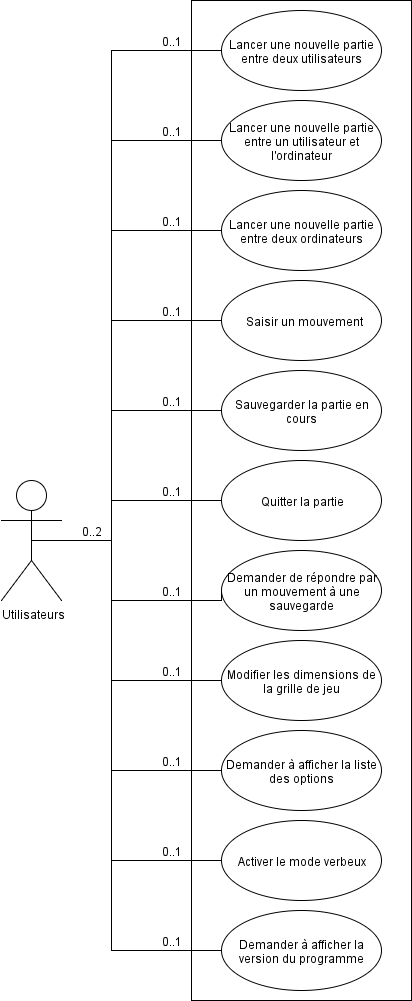
\includegraphics[scale=0.5]{images/use_case.png}
\caption{Diagramme de cas d'utilisation.\label{fig:use_case}}
\end{figure}

\section{Besoins non fonctionnels}
\label{sec:besoins_non_fonctionnels}
\begin{itemize} 
\item Rapidité d'exécution : chaque coup doit être exécuté en moins d'une seconde.
\item Portabilité : le programme doit pouvoir s'exécuter sur toute machine de type Linux.
\end{itemize}

\section{Tests}
\label{sec:tests}

\begin{description}
\item [Sauvegarde et chargement :] La sauvegarde et le chargement d'une partie est testée en vérifiant qu'après la sauvegarde d'une partie, le fichier \verb!ASCII! généré est bien conforme aux conventions précédemment citées (voir section \ref{sec:fonctionnalités}). Par la suite, nous vérifions qu'après le chargement de ce même fichier, la partie possède un plateau de jeu identique à la partie sauvegardée et que le tour du joueur est correct.
\item [Rapidité de l'IA :] La fonction permettant à l'IA d'effectuer un mouvement est soumise à un timeout de une seconde pour assurer que l'IA respecte la contrainte de temps imposée.
\item [Non-régression d'une IA :] Pour s'assurer de la non régression d'une IA, nous affronterons l'IA a son ancienne version.
\end{description}


\section{Gantt}

\begin{center}
\begin{tabular}{| l | c | c | c | c | c | c | c | c | c | c | c | c |}
\hline
Semaines     & 06 & 07 & 08 & 09 & 10 & 11 & 12 & 13 & 14 & 15  \\ \hline
Game         & X  &    &    &    &    &    &    &    &    &     \\ \hline
Board        & X  &    &    &    &    &    &    &    &    &     \\ \hline
Input/Output &    & X  &    &    &    &    &    &    &    &     \\ \hline
Player       &    & X  &    &    &    &    &    &    &    &     \\ \hline
Game Tree    &    &    & X  & X  &    &    &    &    &    &     \\ \hline
Heuristic    &    &    &    &    &  X & X  & X  & X  & X  & X   \\ \hline
\end{tabular}
\end{center}
\newpage

\section{Bibliographie}

\bibliographystyle{alpha}
\bibliography{reversi}{}
\nocite{*}

\end{document}
